\chapter{Conceptos importantes} % Main appendix title
\label{appendix:keyconcepts} % For referencing this appendix elsewhere, use \ref{AppendixA}

La mayor parte de este apéndice se basa en contenido expuesto en \cite{deeplearning}, y son conceptos que el autor considera pertinentes conocerlos de manera que se comprenda de manera adecuada el mundo del \glsentrylong{machinel}.

\section{Capacidad, \glsentrylong{overfitting} y \glsentrylong{underfitting}}
% \todo[inline]{Por hacer, pagina 107 Deep Learning}
El reto central de \gls{machinel} es que nuestro algoritmo tenga un buen rendimiento sobre datos nuevos, entradas nunca antes vistas, no solo las entradas con las que entrenamos nuestro modelo. La habilidad de tener un buen rendimiento sobre nuevos datos se le llama \newterm{generalización}.

Típicamente cuando entrenamos un modelo de \gls{machinel} debemos acceder a un conjunto de entrenamiento; podemos computar una medida de error sobre el conjunto de entrenamiento, llamado el \newterm{error de entrenamiento}; y reducimos este error de entrenamiento. El \newterm{error de generalización} se define como el valor esperado de error sobre una nueva entrada de datos. Aquí el valor esperado se toma sobre diferentes entradas posibles, tomadas de una distribución de entradas que esperamos que el sistema se encontrara en la practica.

Usualmente el error de generalización de un modelo de \gls{machinel} se estima por su rendimiento en un \newterm{conjunto de prueba} que se obtuvieron de manera separada al conjunto de entrenamiento.

El conjunto de datos de entrenamiento y de prueba son generados por una distribucion de probabilidad sobre los conjuntos de datos llamado el \newterm{proceso de generación de datos} (o \textsl{data-generating process} en inglés).

Por lo general asumimos una serie de suposiciones (llamadas usualmente en inglés como \textsl{i.i.d. assumptions}), y es que una muestra de cada conjunto de datos es \newterm{independiente} una de otra y que los conjuntos de entrenamiento y prueba son \newterm{distribuidos idénticamente} tomados de la misma distribución de probabilidad. Esta suposición nos permite describir el proceso generativo de datos con una distribución de probabilidad sobre una sola muestra. Esta misma distribución es luego usada para generar cualquier muestra de entrenamiento y prueba. Llamamos a esta distribución compartida la \newterm{distribución generadora de datos} (o \textsl{data-generating distribution} en inglés), denotada como $\pdata$.

Cuando usamos una algoritmo de \gls{machinel}, no establecemos los parámetros de antemano para luego tomar muestras de ambos conjuntos de datos. Tomamos muestras del conjunto de entrenamiento, luego ajustamos los parámetros para reducir el error en el conjunto de entrenamiento, y luego tomamos muestras del conjunto de prueba. Bajo este proceso, el valor esperado de error en el conjunto de prueba es igual o mayor al del conjunto de entrenamiento. Los factores que determinan que tan bien un algoritmo de \gls{machinel} se desempeñara son su habilidad para
\begin{itemize}
\item Hacer que el error en el conjunto de entrenamiento sea pequeño.
\item Hacer que la diferencia entre el error de prueba y de entrenamiento sea pequeño.
\end{itemize}

Estos dos factores corresponden a los dos grandes retos en \gls{machinel}: \newterm{\gls{underfitting}} y \newterm{\gls{overfitting}}. \gls{underfitting} es cuando el modelo no es capaz de obtener un valor de error suficientemente bajo sobre el conjunto de entrenamiento. \gls{overfitting} ocurre cuando la diferencia entre el valor de error del conjunto de entrenamiento y el conjunto de prueba es muy grande.

Podemos controlar si un modelo es mas propenso a hacer \gls{underfitting} u \gls{overfitting} cambiando su \newterm{capacidad}. Informalmente, la capacidad de un modelo es su habilidad de acomodarse a una gran variedad de funciones. Modelos con baja capacidad pueden tener problemas para adaptarse al conjunto de entrenamiento. Modelos con una alta capacidad pueden adaptarse demasiado por memorizar propiedades del conjunto de entrenamiento que no le son útiles con el conjunto de pruebas.

Una forma de controlar la capacidad de nuestro algoritmo de \gls{machinel} es escogiendo su \newterm{espacio de hipótesis}, el conjunto de funciones que el algoritmo de aprendizaje se le es permitido tomar como función solución.

Un ejemplo de esto es regresión lineal, y es que podemos permitir que nuestro algoritmo de aprendizaje en vez de tomar funciones lineales (de grado $p=1$, \equationref{eq:linear-function}), también pueda tomar funciones polinomiales (grado $p > 1$, \equationref{eq:poly-function}).

\begin{equation} \label{eq:linear-function}
  \hat{y} = b + wx
\end{equation}

\begin{equation} \label{eq:poly-function}
  \hat{y} = b + \sum_{i=1}^{p} w_i x^i
\end{equation}

En este ejemplo, es útil mencionar que existe un teorema que dictamina que para cualquier entero $n \ge 0$ y una lista de $n+1$ puntos en $\R^2$ $(x_0, y_0), \ldots, (x_n, y_n)$, donde $x_0 < x_1 < \cdots < x_n$, existe un polinomio $f$ de grado $n$ tal que $f(x_i) = y_i$ para todo $i$ \cite[pág 15]{kun_2018}. Análogamente a los algoritmos con una gran capacidad, siempre se tiene una función que se adapta perfectamente a los datos de entrenamiento, sin embargo esta función probablemente no sera útil para los datos de prueba. En la practica no siempre es posible obtener una función que se adapte perfectamente a los datos.

Los algoritmos de \gls{machinel} por lo general se desempeñan mejor cuando su capacidad es apropiada para la verdadera complejidad de la tarea que se necesita desarrollar y la cantidad apropiada de datos de entrenamiento que le son provistos.

\begin{figure}[H]
  \centering
  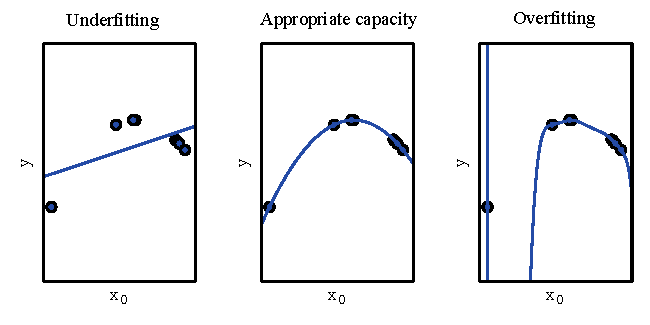
\includegraphics[width=0.9\textwidth]{Figures/capacity-comparison.pdf}
  \decoRule
  \caption[Comparación de capacidades]{Comparación de capacidades. Tomado de \cite{deeplearning}.}
  \label{fig:capacity-comparison}
\end{figure}

Existen muchas maneras de cambiar la capacidad de un modelo, la capacidad no esta solo determinada por la elección del modelo. El modelo especifica cual familia de funciones se pueden escoger cuando se varían los parámetros para alcanzar un objetivo de entrenamiento. A esto se le llama la \newterm{capacidad representativa} (o \textsl{representational capacity} en inglés) del modelo. En muchos casos encontrar la mejor función dentro de esta familia es un problema difícil de optimización. En la practica, el algoritmo de aprendizaje no encuentra la mejor función, sino una que meramente reduce el error de entrenamiento. Estas limitaciones adicionales, tales como la imperfección del algoritmo de optimización, significa que la \newterm{capacidad efectiva} del algoritmo puede ser menor al de la capacidad representativa.

\subsection{Teorema ``No free lunch''}
La teoría de aprendizaje dice que un algoritmo de \gls{machinel} puede generalizar de manera aceptable a partir de un numero finito de muestras de conjuntos de entrenamiento. Esto parece contradecir algunos principios básicos de la lógica. Inferir reglas generales de un conjunto de muestras limitadas no es lógicamente valido. Para inferir lógicamente una regla para describir cada miembro de un conjunto es necesario tener información de todos los miembros de ese conjunto.

\gls{machinel} evita es problema por medio de ofrecer reglas probabilísticas, en vez de ofrecer reglas completamente ciertas como las que ofrece el razonamiento lógico. \gls{machinel} promete encontrar reglas que son \textit{probablemente} ciertas para la \textit{mayor} parte de los miembros de un conjunto que les concierne.

Desafortunadamente, esto no resuelve el problema completo. Existe un teorema llamado ``no free lunch'' el cual afirma que, promediando sobre todas las posibles distribuciones generadoras de datos, cualquier algoritmo de clasificación tiene la misma tasa de error cuando clasifica puntos antes no vistos. Esto quiere decir que no existe un algoritmo de \gls{machinel} que es mejor universalmente a los demás.

Sin embargo, esto solo es aplicable cuando se habla del promedio de \textit{todas} las posibles distribuciones generadoras de datos. Si hacemos suposiciones sobre los tipos de distribución de probabilidad que nos encontramos en la vida real, entonces podemos diseñar algoritmos de aprendizaje que se desempeñan mejor sobre esas distribuciones.

Esto significa que el objetivo de la investigación en \gls{machinel} no busca encontrar un algoritmo de aprendizaje universal, sino que el objetivo es encontrar que tipos de distribuciones son relevantes al ``mundo real'' que un agente de \gls{ai} experimenta, y que tipos de algoritmos de \gls{machinel} se desempeñan bien con datos tomados del tipo de distribuciones generadoras de datos que nos interesan.

\subsection{Regularización}
El teorema de ``no free lunch'' nos dice que debemos diseñar nuestro algoritmo de \gls{machinel} para tener un buen rendimiento en una tarea especifica, esto lo logramos por medio de tener una serie de preferencias dentro del algoritmo de aprendizaje, cuando estas preferencias se alinean hacia el objetivo que queremos lograr este tiene un mejor desempeño.

Aunque una forma de lograr ese objetivo se puede conseguir en parte por medio de modificar la capacidad, no es la única forma de lograrlo. El comportamiento de nuestro algoritmo esta fuertemente influenciado no solo por que tan grande hacemos el conjunto de funciones permitido en su espacio hipótesis, sino también la identidad especifica de esas funciones.

Un método popular para realizar un ajuste de forma que se controle el \gls{underfitting} y el \gls{overfitting} es por medio de modificar nuestra función de costo $J$ agregándole un hiper-parámetro $\lambda$ que se establece de antemano sobre el algoritmo de manera \textit{heurística}. Modificamos $J$ de manera que cuando $\lambda = 0$ no se modifique el valor original de $J$, permitiéndonos controlar el nivel de \gls{underfitting} y \gls{overfitting} con el valor de $\lambda$.

De manera mas general, podemos regularizar un modelo que aprende una función $f(\vx, \vtheta)$ por medio de añadir una penalidad llamada \newterm{regulador} (o \textsl{regularizer} en inglés) a la función de costo $J$. Como ejemplo, téngase una función hipótesis $\hat{f}(\vx, \vtheta) = \vtheta^{\top} \vx$ con parámetros $\vtheta$ y una función objetivo $f(\vx)$ de manera que podemos definir una función de costo que queremos minimizar como:
\begin{equation}
  J(\vx, \vtheta) = | \hat{f}(\vx, \vtheta) - f(\vx) |
\end{equation}

Agregando el regulador $\Omega(\vtheta) = \lambda \vtheta^{\top} \vtheta $ a la función de costo, la ecuación resulta ser
\begin{equation}
  J(\vx, \vtheta) = | \hat{f}(\vx, \vtheta) - f(\vx) | + \Omega(\vtheta)
\end{equation}

De esta manera penalizamos los valores grandes de $\vtheta$ (cuando $\lambda > 0$) que pueden ocasionar \gls{overfitting} de forma que regularizan el avance del algoritmo de optimización que se usa para minimizar la función de costo. Sin embargo, un valor muy grande en $\lambda$ ocasionara \gls{underfitting}.

\begin{figure}[H]
  \centering
  \begin{tabular}{ccc}
    Underfitting          & Appropriate regularization & Overfitting \\
    (Excessive $\lambda$) & (Medium $\lambda$)         & ($\lambda \to 0$) \\
    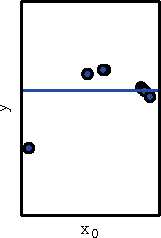
\includegraphics[width=0.25\textwidth]{Figures/regularization-comparison0.pdf} & %
    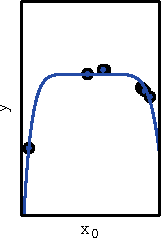
\includegraphics[width=0.25\textwidth]{Figures/regularization-comparison1.pdf} & %
    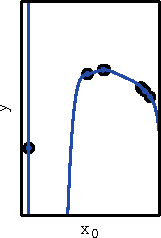
\includegraphics[width=0.25\textwidth]{Figures/regularization-comparison2.pdf} \\
  \end{tabular}
  \decoRule
  \caption[Comparación de valores de regularización]{Comparación de valores de regularización. Tomado de \cite{deeplearning}.}
  \label{fig:regularization-comparison}
\end{figure}

% ================================================================
% ================================================================

\section{Hiper-parámetros y conjuntos de Validación}
% \todo[inline]{Por hacer, pagina 117 Deep Learning}
La mayor parte de los algoritmos de \gls{machinel} tienen hiper-parámetros, que son configuraciones que se pueden usar para controlar el comportamiento del algoritmo. Los valores de los hiper-parámetros no esta controlados por el algoritmo en si mismo.

Algunas veces una configuración se decide poner como un hiper-parámetro que el algoritmo no aprende debido a que la configuración es difícil de optimizar. Es mas común encontrar que la configuración debe ser un hiper-parámetro debido a que no es apropiado ajustarlo con un conjunto de entrenamiento. Esto aplica para todos los hiper-parámetros que controlar la capacidad de un modelo. Si se aprendiera sobre un conjunto de entrenamiento, veríamos que siempre se escogerían hiper-parámetros que llegarían a la capacidad mas alta que sea posible para el modelo, dando como resultado \gls{overfitting}.

Para resolver este problema, necesitamos de un \newterm{conjunto de validación} que el algoritmo de aprendizaje no pueda observar.

Es importante que el conjunto de pruebas no sea usado para ajustar de ninguna manera los parámetros e hiper-parámetros del modelo, de esta manera la forma en que construimos el conjunto de validación es a partir del conjunto de entrenamiento. Específicamente, separamos los datos de entrenamiento en dos conjuntos disyuntos, uno de estos es para aprender los parámetros del modelo; el otro es nuestro conjunto de validación, usado para estimar nuestro error de generalización durante o después del entrenamiento, permitiendo que lo hiper-parámetros sean ajustados adecuadamente. Después de que la optimización de nuestros hiper-parámetros este completa, podemos estimar el error de generalización de nuestro modelo con el conjunto de pruebas.

\subsection{Validación cruzada}
Dividir el conjunto de datos en un conjunto de entrenamiento y pruebas fijo puede ser problemático si resulta que el conjunto de pruebas es pequeño. Un conjunto de pruebas pequeño implica incertidumbre estadística sobre el valor estimado del error de prueba promedio, haciendo difícil decir que un algoritmo A es mejor que el algoritmo B en una tarea especifica.

Cuando el conjunto de datos es muy pequeño, procedimientos alternativos nos permiten utilizar todas las muestras en la estimación del error de prueba promedio, al precio de mayor costo computacional. Estos procedimientos se basan en la idea de repetir las computaciones de entrenamiento y de prueba sobre diferentes subconjuntos escogidos aleatoriamente, o bien divisiones del conjunto de datos original. El procedimiento mas común el de validación cruzada de $k$ partes (conocido como \textsl{$k$-fold cross-validation} en inglés), en donde una partición del conjunto de datos se construye por medio de dividirlo en $k$ subconjuntos disyuntos. El error de prueba se estima por medio de tomar el promedio del error de prueba de todas las $k$ pruebas.

% ================================================================
% ================================================================

\section{Estimadores, Parcialidad (\glsentrylong{bias}) y Varianza}
% \todo[inline]{Por hacer, pagina 119 Deep Learning}
El campo de las estadísticas nos da muchas herramientas para conseguir nuestro objetivo de \gls{machinel} de resolver una tarea no solo con el conjunto de entrenamiento sino que también para generalizar. Conceptos fundamentales como la estimación de puntos, la parcialidad y la varianza son útiles para caracterizar formalmente las nociones de generalidad, \gls{underfitting} y \gls{overfitting}.

\subsection{Estimación de puntos}
La estimación de puntos es el intento de proveer la única ``mejor'' predicción de alguna cantidad de interés. En general esta cantidad de interés puede ser un único parámetro o un vector de parámetros en algún modelo paramétrico.

Para distinguir estimados de parámetros de su valor real se utiliza la distinción de un parámetro $\vtheta$ con $\hat{\vtheta}$.

Sea $\{ \vx^{(1)}, \ldots, \vx^{(m)} \}$ un conjunto de $m$ puntos de datos independientes e idénticamente distribuidos. Un \newterm{estimador} o \newterm{estadístico} es cualquier función en base a los datos:
\begin{equation}
  \hat{\vtheta}_m = g( \vx^{(1)}, \ldots, \vx^{(m)} )
\end{equation}

Sin embargo, la definición no requiere que $g$ sea una buena estimación del verdadero $\vtheta$ ni tampoco que la respuesta este en el mismo conjunto de valores validos de $\vtheta$. Esta definición supone una gran flexibilidad para definir un estimador, sin embargo un buen estimador es una función cuya salida sea cercana al verdadero $\vtheta$ que genero los datos de entrenamiento.

Podemos asumir (desde la perspectiva de estadístico frecuentista) que el valor verdadero del parámetro $\vtheta$ es fijo pero desconocido, y que $\hat{\vtheta}$ es una estimación en función a los datos.

\subsubsection{Estimación de funciones}
La estimación de puntos también puede hacer referencia a la estimación de la relación entre variables entrada y objetivo, nos referimos a estos tipos de estimación de puntos como estimación de funciones.

En este escenario tratamos de predecir una variable $\vy$ dado un vector de entrada $\vx$. Asumimos que existe una función $f(\vx)$ que describe una relación aproximada entre $\vy$ con $\vx$. Podemos asumir que $\vy = f(\vx) + \vepsilon$, donde $\vepsilon$ es la parte de $\vy$ que no es predecible a partir de $\vx$. En la estimación de funciones nos interesa aproximar $f$ con un modelo o estimado $\hat{f}$.

\subsection{Parcialidad (\glsentrylong{bias})}
La parcialidad (o \gls{bias} en inglés) es un estimador definido como:
\begin{equation}
  \mathrm{bias}(\hat{\vtheta}_m) = \E(\hat{\vtheta}_m) - \vtheta
\end{equation}

Donde el valor esperado es sobre los datos (vistos como muestras de una variable aleatoria), donde $\vtheta$ es el valor verdadero de $\vtheta$ usado para definir la distribución que genera los datos. Un estimador se dice que es imparcial (o \textsl{unbiased} en inglés) si $\mathrm{bias}(\hat{\vtheta}_m) = \vzero$, lo cual implica que $\E(\hat{\vtheta}_m) = \vtheta$. Un estimador se dice que es \newterm{asintótico imparcial} si $\lim_{m\to\infty}\mathrm{bias}(\hat{\vtheta}_m) = \vzero$.

Los estimadores imparciales son ciertamente deseables, sin embargo no son siempre los ``mejores'' estimadores.

\subsection{Varianza y Error Estándar}
Otra propiedad de un estimador que puede que debamos tener en cuenta, es que tanto se espera que van a variar nuestros resultados como función de la muestra de datos.

La \newterm{varianza} de un estimador se define como:
\begin{equation}
  \Var(\hat{\rvtheta})
\end{equation}

donde la variable aleatoria $\hat{\rvtheta}$ es el conjunto de entrenamiento. De manera alternativa la raíz cuadrada de la varianza es el \newterm{error estándar}, denotado como $\standarderror(\hat{\rvtheta})$.

La varianza (o el error estándar) de un estimador nos provee de una medida de como esperaríamos que el estimado que computamos de los datos variara cuando retomamos una muestra independiente del conjunto de datos. De la misma manera en que nosotros querríamos una parcialidad baja, querríamos también una varianza baja.

El error estándar de la media esta dado por:
\begin{equation}
  \standarderror(\hat{\mu}_m) = \sqrt{ \Var{\Bigg[ \frac{1}{m} \sum_{i=1}^{m} x^{(i)} \Bigg]} } = \frac{\sigma}{\sqrt{m}}
\end{equation}
    
La varianza de un estimador disminuye en función de $m$, el numero de muestras de nuestro conjunto de datos.

\subsection{Consistencia} \label{app:consistency}
En la labor de escoger un mejor estimador nos interesa especialmente como este se comportara a medida que la cantidad de datos de entrenamiento aumenta. En particular nos interesa que a medida que la cantidad de datos aumenta nuestros estimados se aproximan cada vez mas al verdadero valor de los parámetros. Formalmente deseamos:

\begin{equation} \label{eq:consistency}
  \plim_{m\to\infty} \hat{\rvtheta} = \rvtheta
\end{equation}

El símbolo $\plim$ indica convergencia en probabilidad, indicando que para cualquier $\epsilon > 0$ se tiene que $P(|\hat{\rvtheta} - \rvtheta| > \epsilon) \to 0$ cuando $m \to \infty$. La condición descrita en la \equationref{eq:consistency} se le conoce como \newterm{consistencia}. Algunas veces se le llama consistencia débil, cuando se refiere a consistencia fuerte se hace referencia a la convergencia \textbf{casi segura} de $\hat{\rvtheta}$ a $\rvtheta$. La convergencia casi segura de una secuencia de variables aleatorias $\rvx^{(1)}, \rvx^{(2)}, \ldots$ a un valor $\vx$ ocurre cuando $p(\lim_{m\to\infty}\rvx^{(m)} = \vx) = 1$.

La consistencia nos asegura que la parcialidad inducida por el estimador se elimina a medida que la cantidad de muestras de datos aumenta. Sin embargo lo contrario no es verdad --- imparcialidad asintótica no implica consistencia.

A medida que la capacidad del modelo aumenta, la parcialidad tiende a disminuir y la varianza tiende a aumentar, dándonos así una curva en forma de U para el error de generalización, tal como se muestra en la \figureref{fig:consistency}.

\begin{figure}[H]
  \centering
  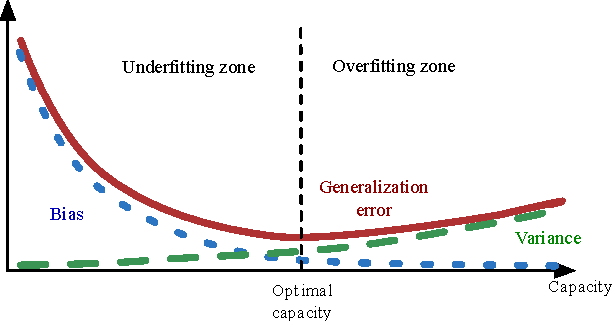
\includegraphics[width=0.7\textwidth]{Figures/consistency.pdf}
  \decoRule
  \caption[Consistencia]{Consistencia. Tomado de \cite{deeplearning}.}
  \label{fig:consistency}
\end{figure}

% ================================================================

\subsection{Estimación de máxima probabilidad} \label{app:maximum-likelihood}
% Pagina 128 Deep Learning
En vez de adivinar si una función se comportara como un buen estimador y luego analizar su parcialidad y su varianza, querríamos tener un principio del cual pudiéramos derivar funciones especificas que son buenos estimadores para modelos diferentes.

Uno de estos principios es el de la estimación de máxima probabilidad (o \textsl{\glsentrylong{mle}} en inglés).

Considérese un conjunto de $m$ muestras $\sX = \{ \vx^{(1)}, \ldots, \vx^{(m)} \}$ tomadas de manera independiente de una distribución generadora de datos $\pdata(\rvx)$ verdadera pero desconocida.

Sea además $\pmodel(\rvx; \vtheta)$ una familia paramétrica de distribuciones de probabilidad sobre el mismo espacio que $\vtheta$. O en otras palabras, $\pmodel(\vx; \vtheta)$ mapea cualquier configuración $\vx$ a un numero real que estima la probabilidad verdadera $\pdata(\vx)$.

El estimador de máxima probabilidad para $\vtheta$ es definido como
\begin{equation}
  \vtheta_{\mathrm{ML}} = \argmax_{\vtheta} \pmodel(\sX; \vtheta) = \argmax_{\vtheta} \prod_{i=1}^{m} \pmodel(\vx^{(i)}; \vtheta)
\end{equation}

Debido a que se trata de probabilidades, se generan varios problemas a la hora de utilizarlo. Las probabilidades al estar en un intervalo de $[0, 1]$, al multiplicarse muchas probabilidades eso puede generar un problema llamada \newterm{underflow}, en la que el hecho de que un numero se acerque demasiado al cero provoca que en la representación interna del computador se trunque a $0$ perdiendo una precisión considerable. Como se trata de una maximizaron de valores, hacer una modificación a la función de costo no cambia el valor objetivo, por lo que podemos aplicarle la función logaritmo a la función de costo, de esta manera reducimos considerablemente el problema de underflow, dejando ahora el único problema al que nos enfrentamos conocido como \newterm{overflow}. La ecuación queda como
\begin{equation}
  \vtheta_{\mathrm{ML}} = \argmax_{\vtheta} \sum_{i=1}^{m} \log \pmodel(\vx^{(i)}; \vtheta)
\end{equation}

Pasando el nombre a ser estimación de máxima probabilidad logarítmica (o \textsl{maximum log-likelihood} en inglés).

\subsubsection{Propiedades de estimación de máxima probabilidad}
Bajo las condiciones apropiadas, el estimador de máxima probabilidad tiene la propiedad de consistencia (véase la \sectionref{app:consistency}), por lo que a medida que el numero de muestras se aproxima a infinito, el estimado de un parámetro converge al verdadero valor, dándonos las siguientes condiciones:
\begin{itemize}
\item La distribución verdadera $\pdata$ debe estar en la familia de modelos $\pmodel(\cdot; \vtheta)$.
  \item La verdadera distribución de $\pdata$ debe corresponder a exactamente un valor para $\vtheta$. De lo contrario, el estimador de máxima probabilidad puede recuperar una distribución $\pdata$ correcta, pero no sera capaz de determinar cual valor de $\vtheta$ es el correcto por el proceso generador de datos.
\end{itemize}

% ================================================================
% ================================================================

\section{Métodos de optimización}
\todo[inline]{Por hacer, mirar si incluirlo de verdad.}

\subsection{Gradiente descendiente}
\todo[inline]{Por hacer, pagina 79 Deep Learning}

\subsection{Gradiente descendiente estocástica}
\todo[inline]{Por hacer, pagina 147 y 286 Deep Learning}

\subsection{AdaGrad}
\todo[inline]{Por hacer, pagina 299 Deep Learning}

\subsection{Adam}
\todo[inline]{Por hacer, pagina 301 Deep Learning}


% ================================================================
% ================================================================

\section{Curva \glsentryname{roc} y valor \glsentryname{auc}}
\todo[inline]{Por hacer, usar \cite{Zou2007}, esto se necesitara para los resultados de los experimentos}
\gls{roc} y \gls{auc}
